\chapter[Application à l'analyse descriptive d'un grand corpus]{Application à l'analyse descriptive d'un grand corpus de décisions jurisprudentielles}
\label{chap:demo}
Ce chapitre décrit des résultats statistiques observés sur un corpus de décisions d'appel formé de la base CAPP de la \citet{dila2019capp} (65k décisions en XML) et 10k décisions de cour d'appel de formats divers collectés à partir d'autres sources. La base CAPP fournit un ensemble de méta-données de référence pour chaque décision notamment la juridiction, la date, la ville. De nouvelles décisions y sont régulièrement ajoutées dans le dépôt en ligne \footnote{Le dépot de CAPP est accessible à partir de \url{https://www.data.gouv.fr/fr/datasets/capp/}}. Il est donc facile d'observer la répartition des décisions entre les villes (\figureref{fig:demo:doc-per-city}) et entre les années (\figureref{fig:demo:doc-per-year}).

\begin{figure}[!htb]
	\centering
	\centering
	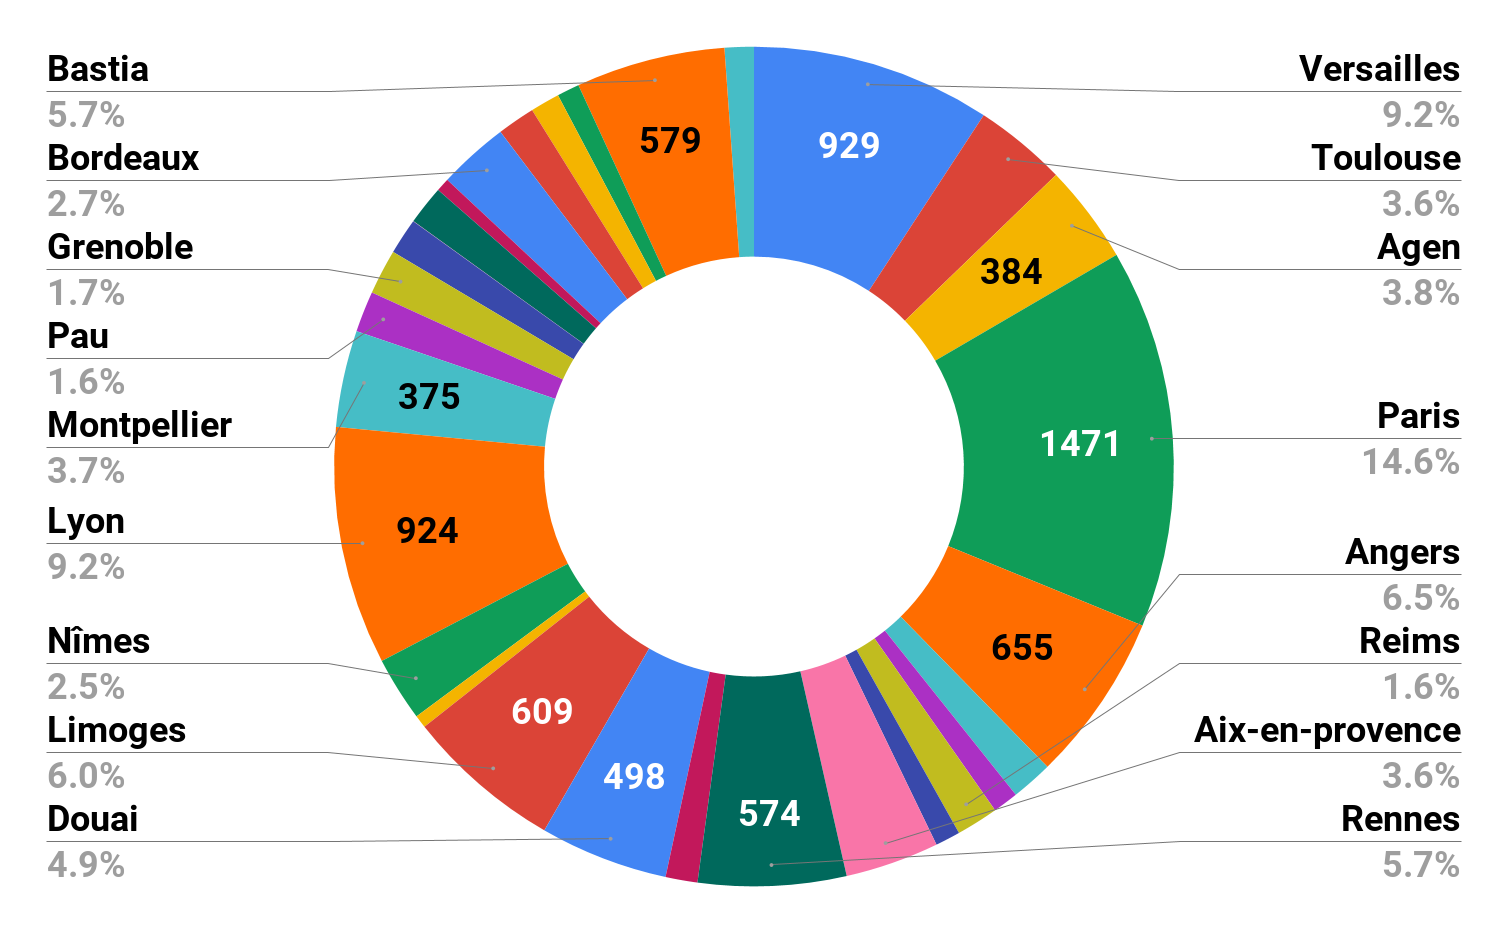
\includegraphics[width=0.9\textwidth]{capp-nbdocparville.png}
	\caption{Répartition des décisions de la base CAPP entre villes.} \label{fig:demo:doc-per-city}
\end{figure}

\begin{figure}[!htb]
	\centering
	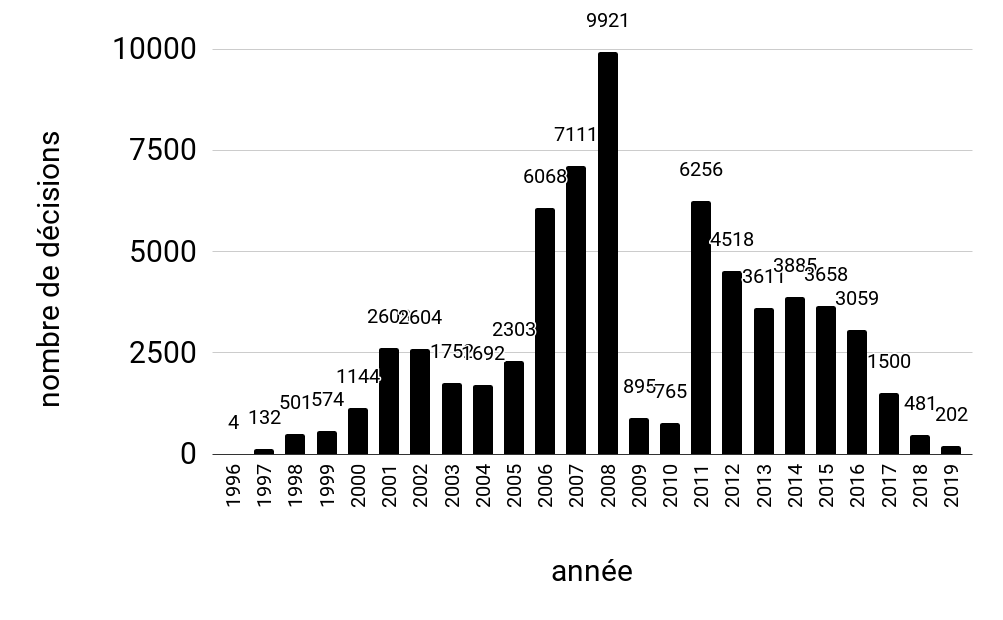
\includegraphics[width=0.9\textwidth]{capp-nbdocparan.png}
	\caption{Nombre de décisions de la base CAPP par année.} \label{fig:demo:doc-per-year}
\end{figure}

 30 villes sont couvertes pour des décisions qui s'étalent entre 1996 et 2019. La répartition n'est pas égale entre les villes.  6 villes ont moins de 100 décisions: Carcassonne (1), Chambéry (50), Nancy (52), Besançon (87), Amiens (97), et Bourges (99). Les cinq (5) villes qui fournissent le plus de décisions fournissent chacune plus de 600 décisions: Paris (14.6\%), Versailles (9.2\%), Lyon (9.2\%), Angers (6.5\%), et Limoges (6.0\%).



La base CAPP couvre par ailleurs des juridictions de nature autre que les cours d'appels qui représentent néanmoins plus de 97\% de CAPP. On y retrouve par exemple des décisions du conseil de prud'hommes, du tribunal de grande instance, du tribunal d'instance, de juridiction de proximité, du Tribunal Supérieur d'Appel, du tribunal de commerce, du tribunal de première instance, etc.


Les connaissances jurisprudentielles ont été extraites à partir de ce corpus non structuré à l'aide des approches proposées dans cette thèse. Après cette extraction, les décisions de la base de données sont réparties entre les villes identifiées automatiquement comme sur la \figureref{fig:demo:doc-per-city} et dans le temps comme sur la \figureref{fig:demo:doc-per-year}. Les demandes extraites se répartissent comme suit: 476 \textit{acpa}, 409 \textit{concdel}, 160 \textit{danais}, 0 \textit{dcppc}, 34 \textit{doris}, et 45928 \textit{styx}.  

%\begin{figure}[ht]
%	\centering
%	\begin{subfigure}[ht]{0.55\textwidth}
%		\centering
%		\centering
%		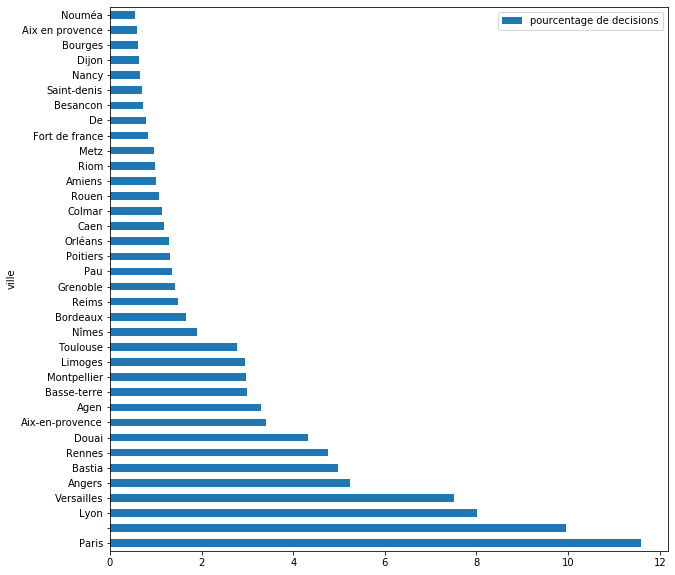
\includegraphics[width=\textwidth]{demo-pourcentage-decision-par-ville.png}
%		\caption{Par ville (pourcentage>0)} \label{fig:demo:doc-per-city}
%	\end{subfigure} 
%	\begin{subfigure}[ht]{0.43\textwidth}
%		\centering
%		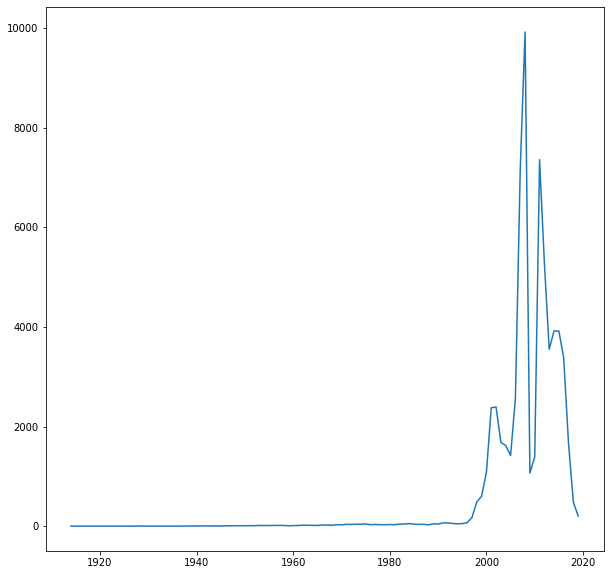
\includegraphics[width=\textwidth]{demo-repartition-decision-par-annee-1900_2019.png}
%		\caption{Par an (entre 1900 et 2019)} \label{fig:demo:doc-per-year}
%	\end{subfigure}
%	\caption{Répartition des décisions} \label{fig:demo:docs-distribution-over-time-and-space}
%\end{figure}


La structuration des données dans la base de données permet de mieux comprendre la jurisprudence à l'aide de graphiques appropriés. Une application de visualisation dédiée a notamment été développée  par \citet{PRYSIAZHNIUK2017jurisprudence-demo-web}.
Les analyses des sections suivantes sont restreintes à 5 villes parmi celles ayant les plus grands nombres de décisions: Paris, Lyon, Versailles, Angers, Bastia; sur la période 2000-2019.

\section{Analyse du sens du résultat}
A partir des données extraites, l'évolution du pourcentage de demandes acceptées  peut être observée sur une courbe. En traçant une telle courbe pour chaque ville, il est possible de comparer les villes.
Par exemple, pour les dommages intérêts sur l'article 700 du Code de Procédure Civile (\textit{styx}), la \figureref{fig:demo:analyse-sens-resultat-styx} compare l'évolution du sens du résultat entre les villes citées précédemment. On remarque que les demandes sont beaucoup plus souvent rejetées qu'acceptées. Pour chaque année, le nombre total de demandes doit être associée pour savoir si le pourcentage de succès est réellement interprétable et comparable à celui des autres années.

\begin{figure}%[!htb]
	\centering 
	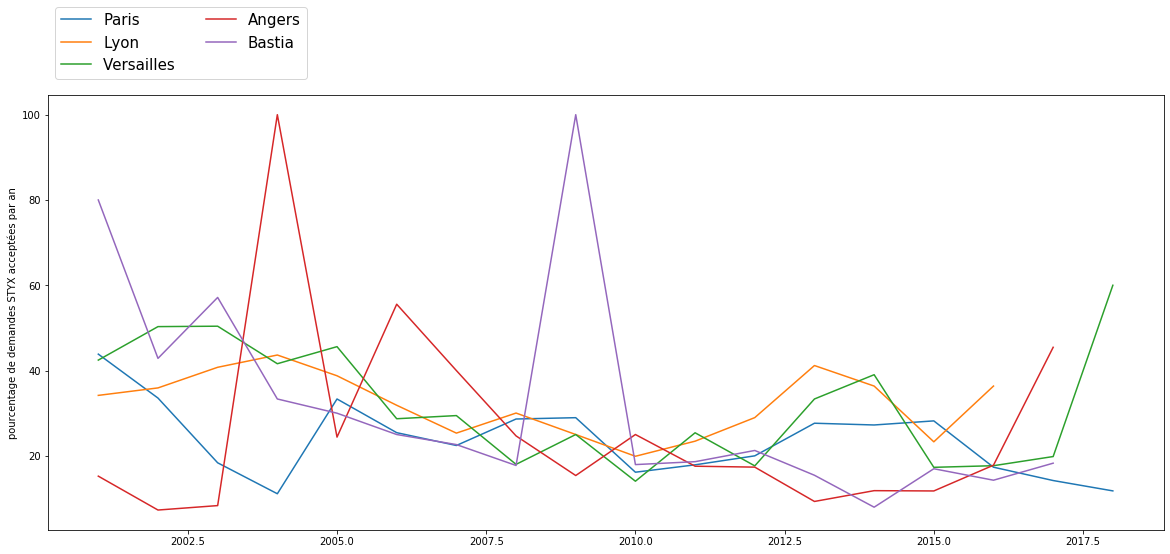
\includegraphics[width=0.8\textwidth]{evolution_sens_resultat_styx.png}
	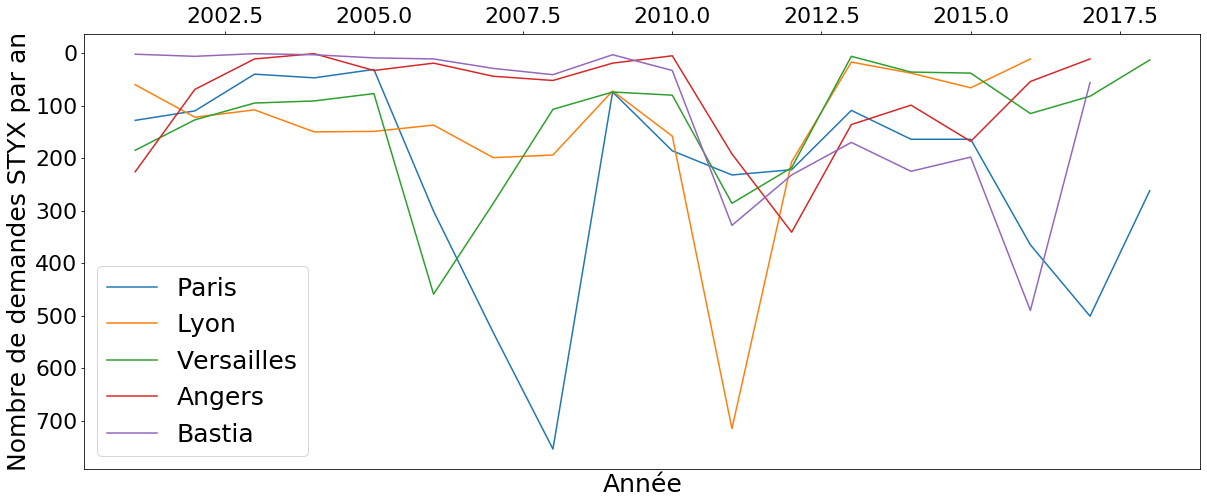
\includegraphics[width=0.8\textwidth]{evolution_nbdmd_styx.png}
	\caption{Evolution du sens du résultat des demandes \textit{styx} dans le temps (années) à Paris, Lyon, Versailles, Angers, Bastia.}\label{fig:demo:analyse-sens-resultat-styx}
\end{figure}

La visualisation par l'application de \citet{PRYSIAZHNIUK2017jurisprudence-demo-web} permet de comparer les villes en observant sur un arbre l'épaisseur des branches associées aux catégories de demande (Figure \figureref{fig:demo:web-styx}). On peut ainsi facilement observer quelles villes acceptent les demandes d'une certaine catégorie plus que d'autres par exemple.

% webdemo-sensresultat-5villes.png

\begin{figure}[!htb]
	\centering 
	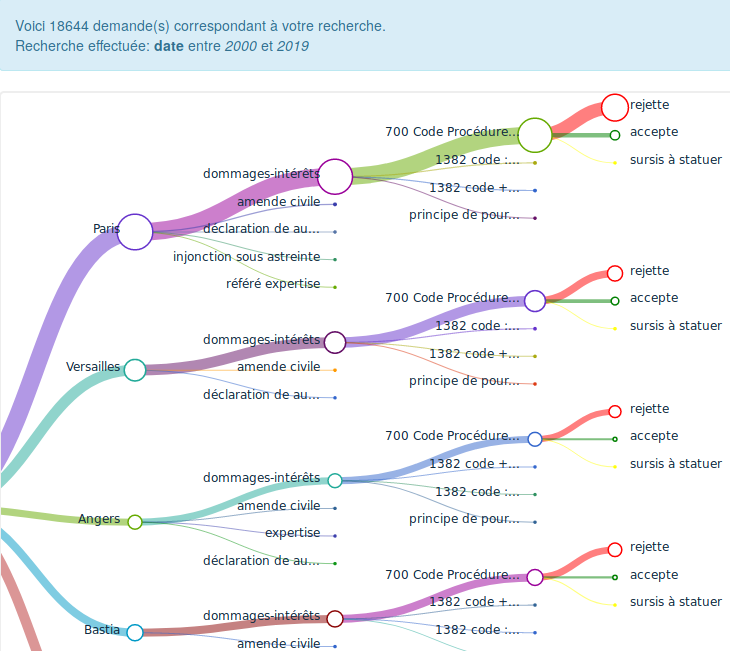
\includegraphics[width=0.6\textwidth]{webdemo-sensresultat-5villes.png}
	\caption{Comparaison de Paris, Lyon, Versailles, Angers, Bastia sur l'acceptation des demandes \textit{styx} à partir d'une visualisation arborée.}\label{fig:demo:web-styx}
\end{figure}

\section{Analyse des quanta}
\subsection{Evolution dans le temps}
\begin{figure}[!htb]
	\centering 
	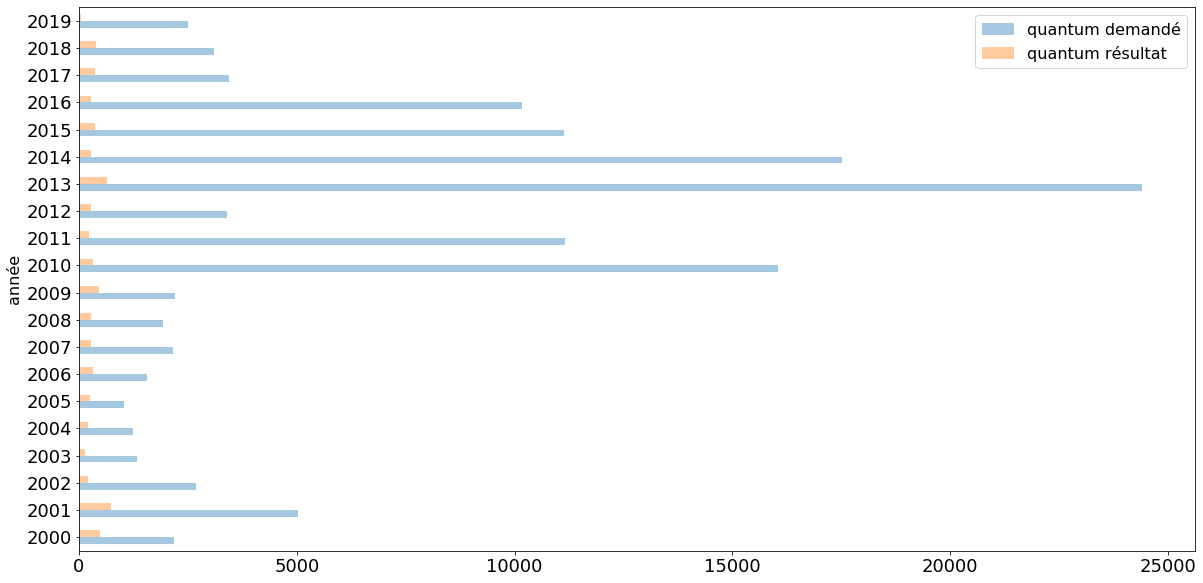
\includegraphics[width=0.8\textwidth]{evolution_quanta_styx.png}
	\caption{Evolution des quanta moyens par année des demandes \textit{styx} entre  2000  et 2019.}\label{fig:demo:evolution-quanta-styx}
\end{figure}

De même l'évolution des quanta demandés et accordés peut être facilement visualisée par un diagramme en barre comme celui de la \figureref{fig:demo:evolution-quanta-styx} qui correspond aux demandes \textit{styx} entre 2000  et 2019. Même si le nombre total de demandes est à prendre en compte, un tel diagramme donne un aperçu des sommes d'argent moyennes demandées et accordées chaque année. Malheureusement, une seule valeur aberrante très élevée a un impact négatif sur l'interprétation de la moyenne. On observe par exemple une moyenne particulièrement haute en 2013  (\figureref{fig:demo:evolution-quanta-styx}). On préfèrera des diagrammes boîtes (\textit{box plot}) comme celui de l'évolution des quanta accordés de moins de 10k \euro{} à Bastia (\figureref{fig:demo:evolution-qr-styx-compare-ville}). Par exemple, même si les médianes en 2001 et 2002 sont presque égales, les quanta accordés non nuls ont été très proches en 2001 par rapport à 2002 où la distribution est plus large.

\subsection{Variabilité dans les territoires}

\begin{figure}[!htb]
	\centering 
	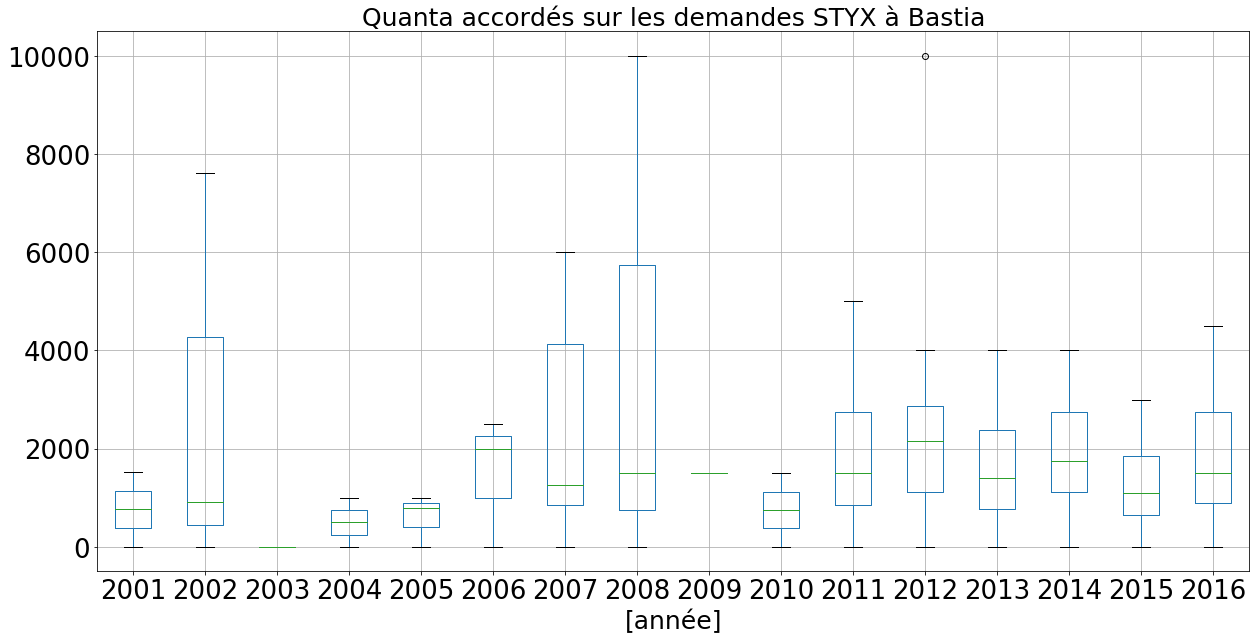
\includegraphics[width=0.8\textwidth]{qr_STYX_Bastia.png}
	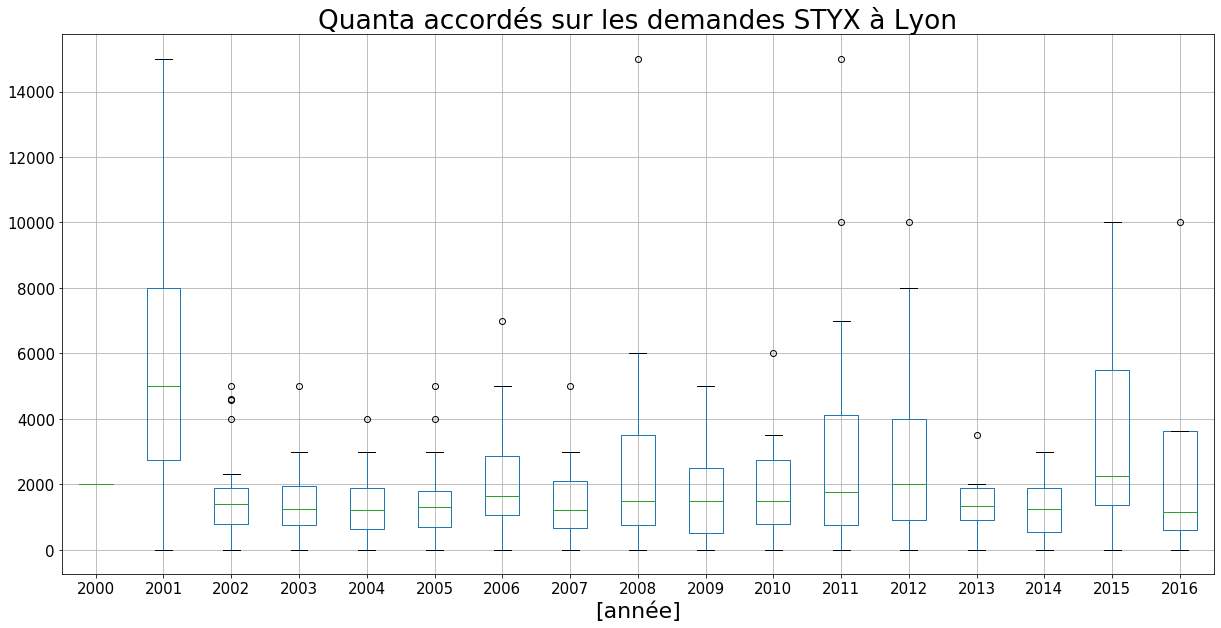
\includegraphics[width=0.8\textwidth]{qr_STYX_Lyon.png}
	\caption{Evolution des quanta accordés (< 10k \euro) par année sur les demandes \textit{styx} entre 2000 et 2016 à Bastia et à Lyon.}\label{fig:demo:evolution-qr-styx-compare-ville}
\end{figure}

Pour avoir une idée du montant que l'on peut recevoir pour une catégorie de demande, l'évolution des valeurs généralement accordées peut être comparée entre deux villes en visualisant les diagrammes boîtes
des quanta accordés dans ces villes. La  \figureref{fig:demo:evolution-qr-styx-compare-ville} permet d'effectuer des comparaisons entre Bastia et Lyon. En 2008 par exemple, les quanta accordés sont plus proches entre eux à Lyon qu'à Bastia.


\subsection{Quantum demandé vs. quantum accordé}
La prédiction du quantum résultat doit définir un modèle dont la forme s'accorde avec celle du nuage de points ($x=$ quantum demandé, $y=$ quantum accordé) correspondant. D'après les nuages de points observés pour Paris, Bastia, Angers et Lyon (\figureref{fig:demo:qr-vs-qd-styx-compare-ville}), le quantum demandé ne semble pas suffisant seul pour déterminer le quantum accordé\footnote{Différentes valeurs de quantum résultat sont observées pour la même valeur de quantum demandé.}. Il sera ainsi nécessaire de tenir compte des circonstances factuelles et autres spécificités du cas traité qui permettront de filtrer les décisions sur lesquelles se basera l'apprentissage. On remarque néanmoins une ressemblance de forme entre les nuages de points des différentes villes. On observe empiriquement une caractéristique du droit qui est \og l'impossibilité d'accorder plus qu'une somme demandée\fg{}.

\begin{figure}[!htb]
	\centering 
	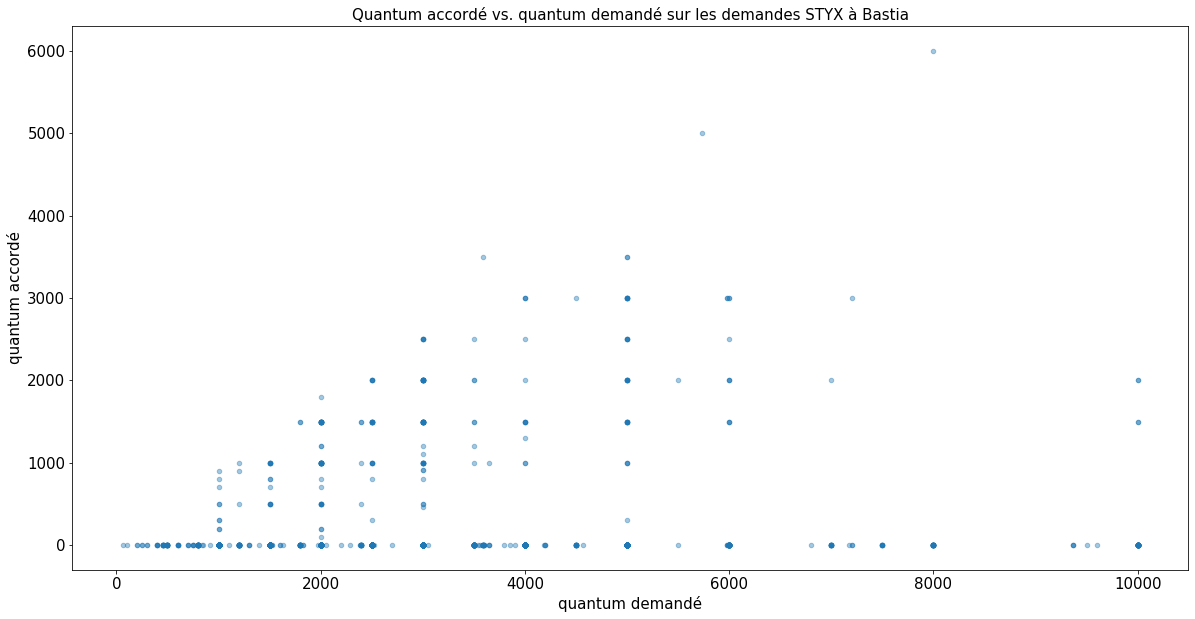
\includegraphics[width=0.47\textwidth]{qr-vs-qd_STYX_Bastia.png}
	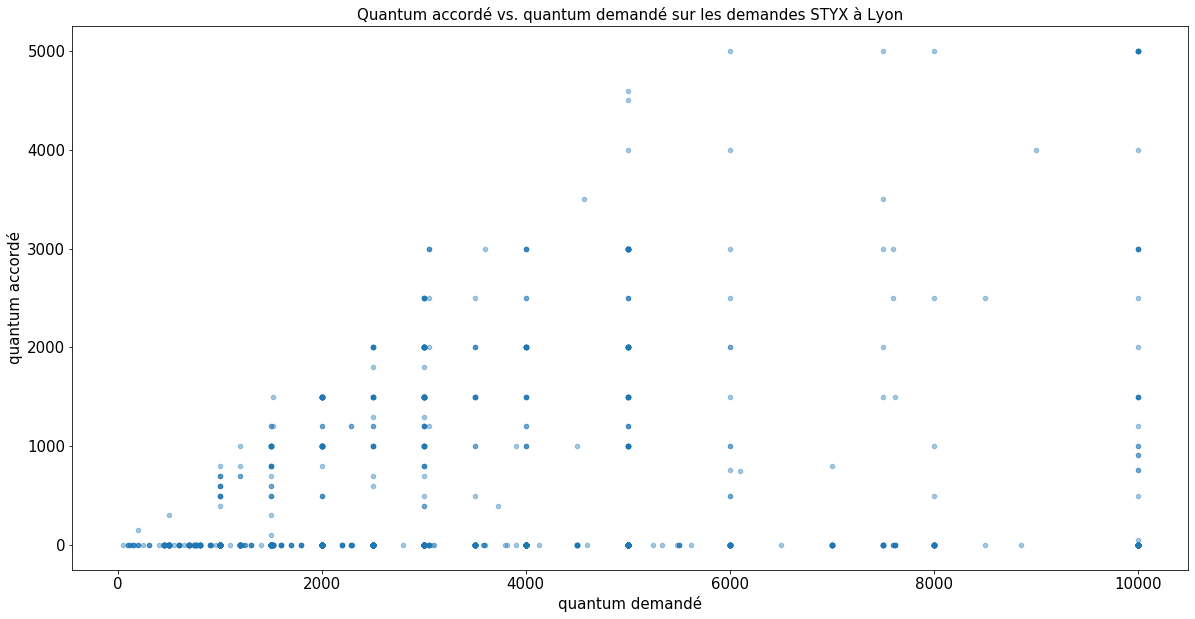
\includegraphics[width=0.47\textwidth]{qr-vs-qd_STYX_Lyon.png}
	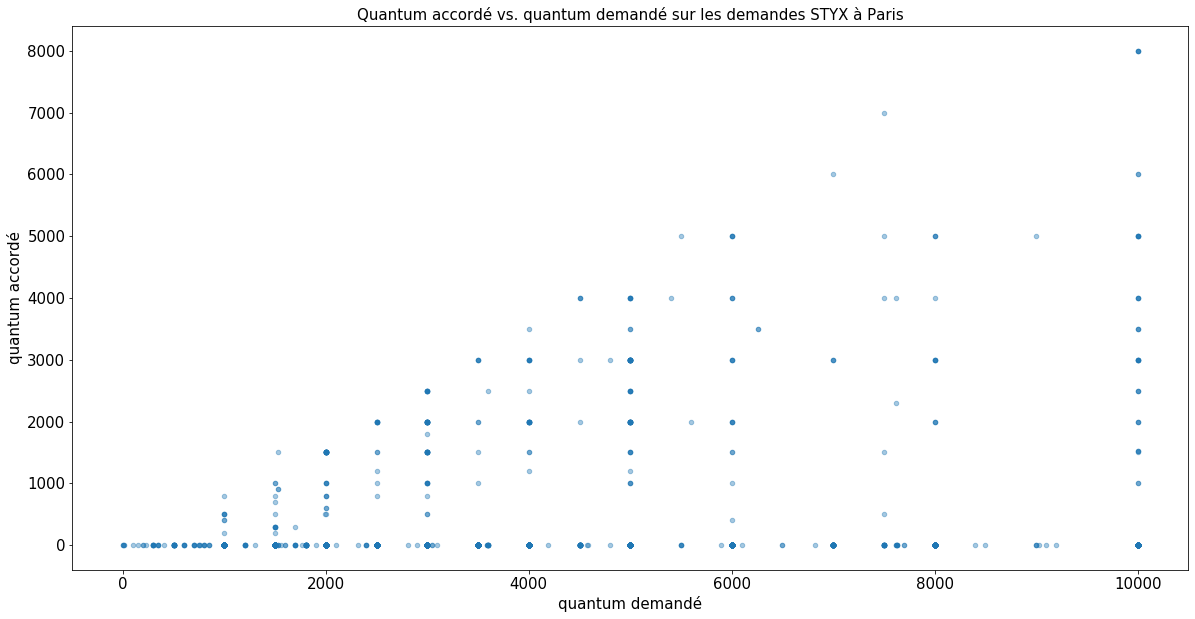
\includegraphics[width=0.47\textwidth]{qr-vs-qd_STYX_Paris.png}
	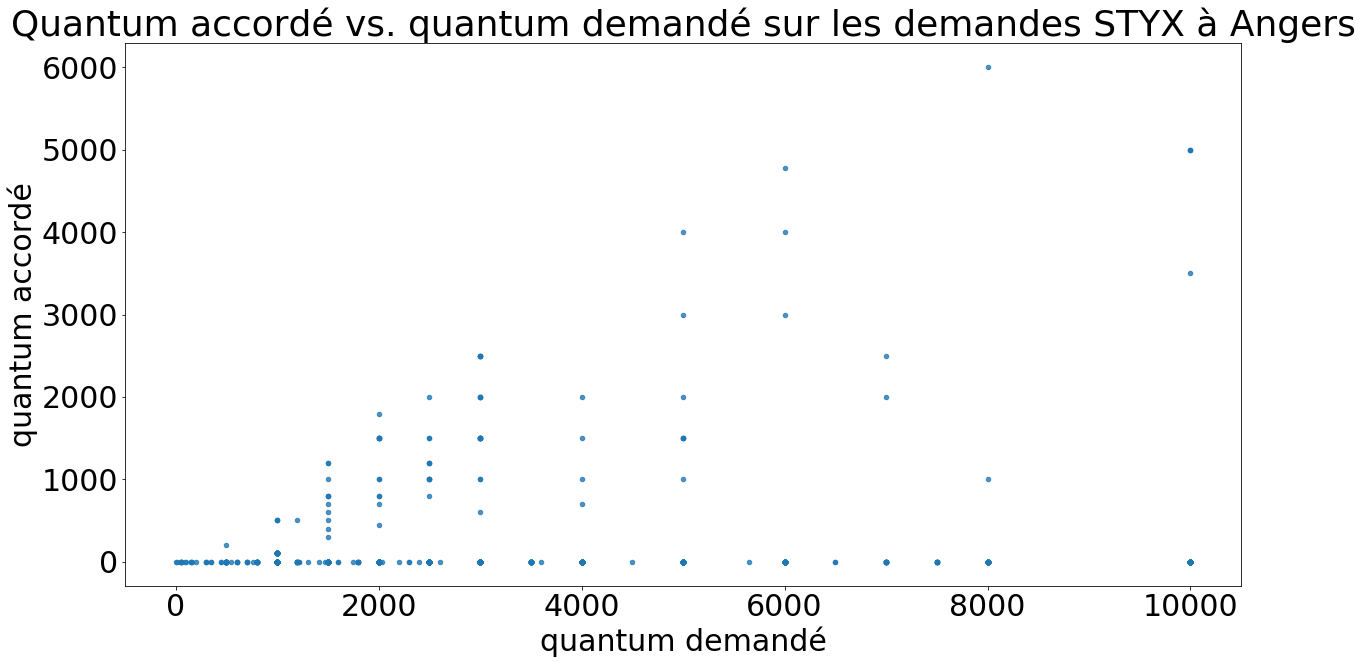
\includegraphics[width=0.47\textwidth]{qr-vs-qd_STYX_Angers.png}
	\caption{Nuages de points (quantum accordé, quantum demandé) pour les demandes \textit{styx} entre 2000 et 2019 à Paris, Bastia, Angers et Lyon (quantum demandé < 10000).}\label{fig:demo:qr-vs-qd-styx-compare-ville}
\end{figure}

\section{Conclusion}
\label{sec:demo:conclusion}
Les démonstrations de ce chapitre donnent quelques exemples de statistiques qui informent de l'état de la jurisprudence à partir d'informations extraites à l'aide des approches proposées dans cette thèse. Les analyses du sens du résultat et des quanta sont les principales applications directes des propositions développées. Ce chapitre se limite aux filtres sur l'année, la ville, et la catégorie de demande, mais les analyses peuvent déjà être affinées en associant d'autres filtres comme  des mot-clés, les normes appliquées, ou le type de juridiction. Les analyses pourront être enrichies grâce l'extraction future de nouvelles informations comme les motivations des juges et de meilleurs modèles d'identification de circonstances factuelles.